\documentclass{article}

%\documentclass{proc-l}

\usepackage{amssymb}
\usepackage{amsmath}
\usepackage{amsfonts}
\usepackage{amsthm}

\usepackage{graphicx}

\newcommand{\C}{\mathcal{C}}
\newcommand{\sN}{\mathcal{N}} 
\newcommand{\M}{\mathcal{M}}
\newcommand{\X}{\mathbf{X}}
\newcommand{\T}{\mathcal{T}}

\newcommand{\vv} {{\boldsymbol{\nu}}}
\newcommand{\x}{{\bf x}}
\newcommand{\xx}{\mathbf{x}}
\newcommand{\be}{{\bf e}}
\newcommand{\ff}{{\mathbb{ F\!}}}
\newcommand{\lff}{{\mathbb{ F\!}}^{\,\prime}}
\newcommand{\pp}{{\mathbb{P\!}}}
\newcommand{\Fq}{{\mathbb{F\!}_q}}
\newcommand{\Fp}{{\mathbb{F\!}_p}}
\newcommand{\FF}{\mathbb{F}_2}
\newcommand{\F}{\mathbb{F}}
\newcommand{\QQ}{\mathbb{Q}_2}
\newcommand{\Qp}{\mathbb{Q}_p}
\newcommand{\Q}{\mathbb{Q}}
\newcommand{\Z}{\mathbb{Z}}
\newcommand{\Zp}{\mathbb{Z}_p}
\newcommand{\K}{K}
\newcommand{\N}{\mathbb{N}}
\newcommand{\p}{$p$\nobreakdash}
%\newcommand{\e}{\mathbf{e}}
\newcommand{\tvec}{\mathbf{t}}
\newcommand{\OKxi}{\mathcal{O}_{\K(\xi)}}
\DeclareMathOperator{\tr}{Tr}
\def\Tr{\mathop{\rm Tr}\nolimits}
\newcommand{\cc}{\mathcal{C}}
\newcommand{\il}{\mathcal{I}}
\newcommand{\ee}{\epsilon}
\newcommand{\bb}{\beta}

%%%%%%%%%%%%%%%%%%%%%%%%
% AMS Proc Styles
%%%%%%%%%%%%%%%%%%%%%%

\newtheorem{theorem}{Theorem}[section]
\newtheorem{lemma}[theorem]{Lemma}

\theoremstyle{definition}
\newtheorem{definition}[theorem]{Definition}

%\theoremstyle{corollary}
\newtheorem{corollary}[theorem]{Corollary}

\newtheorem{example}[theorem]{Example}
\newtheorem{xca}[theorem]{Exercise}

\newtheorem{construction}[theorem]{Construction}


\newtheorem{prop}[theorem]{Proposition}

\theoremstyle{remark}
\newtheorem{remark}[theorem]{Remark}

\numberwithin{equation}{section}




\begin{document}

\title{On a Class of Permutation Polynomials over Finite Fields}

\author{Christian A. Rodriguez Encarnacion \\ Alex D. Santos Sosa \\ Ivelisse Rubio \\ Francis Castro}

\maketitle

\begin{abstract}
Given $q=p^r$, $d_1$ and $d_2$, we construct partitions of polynomials of the form $F_{a,b}(X) =X\left(X^{\frac{q-1}{d_1}} + a X^{\frac{q-1}{d_2}} + b \right)$, where $a,b \in \mathbb{F}_{q}^{*}$, that have value sets of the same cardinality. As a consequence we provide families of permutation polynomials and of polynomials with small value sets. 

%Permutation polynomials over finite fields are important in many applications, for example in coding theory and cryptography. Our goal is to provide families of polynomials that are rich in permutation polynomials, and study polynomials of the form $F_{a,b}(X) =X\left(X^{\frac{q-1}{d_1}} + a X^{\frac{q-1}{d_2}} + b \right)$, where $a,b \in F_{q}$, $q=p^r$, $p$ prime, $d_1 \mid (q-1)$ and $d_2 \mid (q-1)$. We prove that the number of polynomials of the form $F_{a,b}(X)$ with value set of size $\left\vert V_{F_{a,b}} \right\vert =n$ is a multiple of $lcm(d_1,d_2)$ and give a construction where, given a permutation polynomial $F_{a,b}(X)$ of $\mathbb{F}_q$, we can construct a list of $lcm(d_1,d_2)$ coefficients $[a',b']$ such that $F_{a',b'}(X)$ is also a permutation polynomial of $\mathbb{F}_q$.
\end{abstract}


%%%%%%%%%%%%%%%%%%%%%%%%%%%%%%%%%%%%%%%%%%%%%%%%%%%%%%%%%%%%%%%%%%%%%%%
\section{Introduction}
%%%%%%%%%%%%%%%%%%%%%%%%%%%%%%%%%%%%%%%%%%%%%%%%%%%%%%%%%%%%%%%%%%%%%%%

Permutation polynomials over finite fields are important in many applications, for example in cryptography and coding theory. Monomials and binomials that produce permutations have been studied extensively making trinomials the next step to be studied. Our goal is to provide families of polynomials that are rich in permutation polynomials. While experimenting with trinomials, we found that within the family of polynomials of the form $$F_{a,b}(X) = X(X^{\frac{q-1}{d_1}} + aX^{\frac{q-1}{d_2}} +b)$$ where $d_1 | (q-1)$ and $d_2 | (q-1)$  there are many permutation polynomials. In addition to the amount of permutation polynomials this family provides, we also saw interesting patterns in the value sets. We want to find conditions in $a,b$ that guarantee that $F_{a,b}(X)$ is a permutation polynomial and count how many permutation polynomials exist in each family. Also we want to study the relation between the value sets and the permutation polynomials. 

An example of applications of permutation polynomials over finite fields are RSA-type cryptosystems. In some of these systems secret messages are encoded as elements of a field $\mathbb{F}_{q}$ with a sufficiently large $q$. The encryption operator used for these systems is a permutation of the field $\mathbb{F}_{q}$ and needs to be efficiently computable. It is easy to see that expressing this operator in terms of a permutation polynomial is simple and efficient. Polynomials with minimal value sets are related with ellyptic curves with a large number of rational points.

The rest of this report goes as follows: In the preliminaries section we present definitions pertinent to our work. Afterwards, in the following section we present our results related to the value sets of our polynomial $F_{a,b}(X)$. In the next section we talk about our ongoing work and current open problems.

%%%%%%%%%%%%%%%%%%%%%%%%%%%%%%%%%%%%%%%%%%%%%%%%%%%%%%%%%%%%%%%%%%%%%%%
\section{Preliminaries}
%%%%%%%%%%%%%%%%%%%%%%%%%%%%%%%%%%%%%%%%%%%%%%%%%%%%%%%%%%%%%%%%%%%%%%%

\begin{definition}
  A \textbf{permutation} of a set $A$ is an ordering of the elements of $A$. A function $f: A \rightarrow A$ gives a permutation of $A$ if and only if $f$ is one to one and onto.
\end{definition}

We are interested in studying polynomials that permute the elements of a finite field.

\begin{definition}
  A \textbf{finite field} $\mathbb{F}_{q}$, $q=p^r$, $p$ prime, is a field with $q=p^r$ elements.
\end{definition}

\begin{example}
    $\mathbb{F}_7 = {0,1,2,3,4,5,6}$
  \end{example}

An important property across our work is the existence of a primitive root for a finite field. We use primitive roots in many of our proofs.

\begin{definition}
  A \textbf{primitive root} $\alpha \in \mathbb{F}_q$ is a generator for the multiplicative group $\mathbb{F}_{q}^{*}$
\end{definition}

\begin{example}
  Consider the finite field $\mathbb{F}_{7}$. We have that: $3^1 = 3, 3^2 = 2, 3^3 = 6, 3^4 = 4, 3^5 = 5, 3^6 = 1$, so $3$ is a primitive root of $\mathbb{F}_{7}$.
\end{example}

\begin{example}
  Consider $\mathbb{F}_{7}$. Since $2^1 = 2, 2^2 = 4, 2^3 = 1, 2^4 = 2,$ $ 2^5 = 4, 2^6 = 1$, $2$ is not a primitive root of $\mathbb{F}_{7}$.
\end{example}

Because of the patterns in the value sets we mentioned earlier, given a polynomial defined over a finite field, we study the image of this polynomial. We call this image the value set of the polynomial.

\begin{definition}
  Let $f(x)$ be a polynomial defined over a finite field $\mathbb{F}_{q}$. Then the \textbf{value set} of $f$ is defined as $V(f) = Im(f) = \left\{f(a) \mid a \in \mathbb{F}_{q} \right\}$
\end{definition}

\begin{example}
  Consider $f(x) = x^2$ defined over $\mathbb{F}_{5}$. Note: $f(0) = 0, f(1) = 1, f(2) = 4, f(3) = 4, f(4) = 1$, so $V_{f} = \left\{0, 1, 4 \right\}$.
\end{example}

Note that a polynomial $f(x)$ defined over $\mathbb{F}_{q}$ is a permutation polynomial if and only if  $V(f) = \mathbb{F}_{q}$.


\begin{example}
  Consider the polynomial $f(x) = x+3$ defined over $\mathbb{F}_{7}$. We have that $f(0) = 3, f(1) = 4, f(2) = 5, f(3) = 6, f(4) = 0, f(5) = 1, f(6) = 2$, so $f(x)$ is a permutation polynomial over $\mathbb{F}_{7}$
\end{example}

\begin{example}
Let $f(x) = x^2$ over $\mathbb{F}_{5}$. We have that $V_{f} = \left\{0, 1, 4 \right\}$ so $f(x)$ is not a permutation polynomial over $\mathbb{F}_{5}$.
\end{example}

Recall now that we are interested in studying the family of polynomials $F_{a,b}(X) = X(X^{\frac{q-1}{d_1}} + aX^{\frac{q-1}{d_2}} +b)$ defined over $\mathbb{F}_q$ where $d_1 | (q-1)$, $d_2 | (q-1)$ and $a,b \in \mathbb{F}_q^*$. Specifically, we are interested in studying the value set of $F_{a,b}(X)$ given a pair of coefficients $(a,b)$.

%%%%%%%%%%%%%%%%%%%%
\section{Motivation}    
%%%%%%%%%%%%%%%%%%%%

As we stated in the introduction permutation polynomias over finite fields have many applications in cryptography and coding theory but at the same time are a very extense and complicated field of study. Because of that people have decided to study permutation polynomials by . All of the information about Permutation Monomials is known. Binomials that produce permutations of finite fields have also been studied extensively. The next case to be studied are trinomials. We have found that within the family of polynomials of the form $F_{a,b}(X) =X\left(X^{\frac{q-1}{d_1}} + a X^{\frac{q-1}{d_2}} + b \right),$ there are many permutation polynomials. We want to find conditions in $a,b$ that guarantee that $F_{a,b}(X)$ is a permutation polynomial and count how many permutation polynomials exist in each family.

%%%%%%%%%%%%%%%%%%%%
\section{Results}
%%%%%%%%%%%%%%%%%%%%

Given $q$, $d_1$ and $d_2$ the value set of a particular polynomial $F_{a,b}(X)$ is characterized by the pair of coefficients $(a,b)$. In order to simplify notation we use the following definition for value sets.

\begin{definition}
  Let $d_1, d_2 \in \mathbb{F}_q$ be such that $d_1 \mid q$ and $d_2 \mid q$. We define the polynomial $F_{a,b}(x) = x(x^{\frac{q-1}{d_1}} + ax^{\frac{q-1}{d_2}} +b)$ with $a,b \in \mathbb{F}_q^{*}$ and $V(F_{a,b}) = Im(F_{a,b}(x))$.
\end{definition}

For convenience we define a relation in $\mathbb{F}_q^* \times \mathbb{F}_q^*$ between pairs of coefficients $(a,b)$ of $F_{a,b}$. This will allow us to express our results in a simplified notation.

\begin{definition}\label{relacion}

  Let $a = \alpha^i, b = \alpha^j$ and $\sim$ be the relation in $\mathbb{F}_q^* \times \mathbb{F}_q^*$ defined by $(a,b) \sim (a', b')$ 
  $\Longleftrightarrow a' = \alpha^{i+h(\frac{q-1}{d_1} - \frac{q-1}{d_2})}, b' = \alpha^{j+h(\frac{q-1}{d_1})}$, where $h \in \mathbb{Z}$

\end{definition}

 \begin{example}
    Let $q = 13, d_1 = 2, d_2 = 3$, then we have $\alpha = 2$ and take $a = 4 = 2^2, b = 8 = 2^3$. Now $(a,b) \sim (a',b')$ if and only if
    $a' = \alpha^{2+2h}, b' = \alpha^{3+6h}$. In particular $(2,8) \sim (3,5)$
  \end{example}

Our first result provides a solid foundation for our work.

\begin{lemma}
  
  The relation $\sim$ defined in Def~\ref{relacion} is an equivalence relation in $\mathbb{F}_q^* \times \mathbb{F}_q^*$.

\end{lemma}

\begin{proof}
  
  1. Let $a=\alpha^i$, $b=\alpha^j$ and choose $h=0$. Then $a' = \alpha^{i+0(\frac{q-1}{d_1}-\frac{q-1}{d_2})} = \alpha^i = a$ and $b' = \alpha^{j+0(\frac{q-1}{d_1})} = \alpha^j = b$. Therefore $(a,b) \sim (a,b)$ and the relation is reflexive.

  2. Let $a = \alpha^i$, $b=\alpha^j$, $a' = \alpha^{i+h(\frac{q-1}{d_1}-\frac{q-1}{d_2})}$ y $b' = \alpha^{j+h(\frac{q-1}{d_1})}$ then $(a,b) \sim (a',b')$. We want to find $l$ such that $a = \alpha^{i+h(\frac{q-1}{d_1}-\frac{q-1}{d_2})+l(\frac{q-1}{d_1}-\frac{q-1}{d_2})}$ y $b = \alpha^{j+h(\frac{q-1}{d_1})+l(\frac{q-1}{d_1})}$. Choose $l=d_1d_2-h$, then we obtain: $\alpha^{i+d_1d_2(\frac{q-1}{d_1}-\frac{q-1}{d_2})} = \alpha^i = a$ and $\alpha^{j+d_1d_2(\frac{q-1}{d_1})} = \alpha^j = b$. Therefore $(a',b') \sim (a,b) $ and the relation is symmetric.

  3. Suppose that $a = \alpha^i$, $b=\alpha^j$, $a' = \alpha^{i+h(\frac{q-1}{d_1}-\frac{q-1}{d_2})}$, $b' = \alpha^{j+h(\frac{q-1}{d_1})}$, $a'' = \alpha^{i+h(\frac{q-1}{d_1}-\frac{q-1}{d_2})+l(\frac{q-1}{d_1}-\frac{q-1}{d_2})}$, $b'' = \alpha^{j+h(\frac{q-1}{d_1})+l(\frac{q-1}{d_1})}$. Therefore $(a,b) \sim (a',b')$ and $(a',b') \sim (a'',b'')$. Note that $a'' = \alpha^{i+(h+l)(\frac{q-1}{d_1}-\frac{q-1}{d_2})}$, $b'' = \alpha^{j+(h+l)(\frac{q-1}{d_1})}$, therefore $(a,b) \sim (a'',b'')$ and the relation is transitive.

  In conclusion the relation is an equivalence relation.

\end{proof}

The equivalence relation defined in Def~\ref{relacion} induces and equivalence relation in the set of polynomials of the form $F_{a,b}(X) = X(X^{\frac{q-1}{d_1}} + aX^{\frac{q-1}{d_2}} +b)$ with equivalence classes $[F_{a,b}] = [F_{\alpha^i, \alpha^j}] = \left\{\ F_{a',b'} | a' = \alpha^{i+h(\frac{q-1}{d_1} - \frac{q-1}{d_2})}, b' = \alpha^{j+h(\frac{q-1}{d_1})} \right\}$

Given that our relation $\sim$ is an equivalence relation, we study the value set $V(F_{a,b})$ in the context of the equivalence class $[F_{a,b}]$. Our next lemma states that all polynomials belonging to the same equivalence class have value sets of the same size. 

\begin{lemma}
  
  Suppose that $F_{a,b} \sim F_{a',b'}$ where $\sim$ is the relationship defined in Definition~\ref{relacion}. Then $|V(F_{a,b})| = |V(F_{a',b'})|$

\end{lemma}

\begin{proof}
  
  Let $\alpha$ be a primitive root of the finite field $\mathbb{F}_q$. $$F_{a', b'}(\alpha^{k+1}) = \alpha^{k+1}((\alpha^{k+1})^{\frac{q-1}{d_1}} + \alpha^{i + \frac{q-1}{d_1} - \frac{q-1}{d_2}}(\alpha^{k+1})^{\frac{q-1}{d_2}} + \alpha^{j + \frac{q-1}{d_1}})$$

  $$= \alpha^{k+1}((\alpha^{k})^{\frac{q-1}{d_1}} \cdot \alpha^{\frac{q-1}{d_1}} + \alpha^{i} \cdot \frac{\alpha^{\frac{q-1}{d_1}}} {\alpha^{\frac{q-1}{d_2}}} (\alpha^{k})^{\frac{q-1}{d_2}} \cdot \alpha^{\frac{q-1}{d_2}} + \alpha^{j} \cdot \alpha^{\frac{q-1}{d_1}})$$

  $$= \alpha^{\frac{q-1}{d_1} + 1} \cdot \alpha^{k}((\alpha^{k})^{\frac{q-1}{d_1}} + \alpha^{i}(\alpha^{k})^{\frac{q-1}{d_2}} + \alpha^{j} )$$

  $$= C \cdot F_{a,b}(\alpha^k), \mbox{where } C = \alpha^{\frac{q-1}{d_1} + 1}$$

  In general for each element $\alpha^{\frac{q-1}{d_1} + 1}F_{a,b}(\alpha^{k})$ there will be a corresponding element $F_{a',b'}(\alpha^{k+1})$ where $a' = \alpha^{i + h(\frac{q-1}{d_1} - \frac{q-1}{d_2})}$ y $b'= \alpha^{j + h(\frac{q-1}{d_1})}$. We can then define a function $f:V(F_{a',b'}) \rightarrow \alpha^{\frac{q-1}{d_1}}V(F_{a,b})$ by $f(F_{a', b'}(\alpha^{k+1})) = \alpha^{\frac{q-1}{d_1}+1}F_{a, b}(\alpha^k)$. We prove that $f$ is one to one.


  Suppose that $f(F_{a', b'}(\alpha^{k_1+1})) = f(F_{a', b'}(\alpha^{k_2+1}))$ where $k_1, k_2 \in \mathbb{F}_q$. Consider $f(F_{a', b'}(\alpha^{k_1+1}))$

  $$= f(\alpha^{k_1+1}((\alpha^{k_1+1})^{\frac{q-1}{d_1}} + \alpha^{i}(\alpha^{k_1+1})^{\frac{q-1}{d_2}} + \alpha^{j}))$$ 

  $$= \alpha^{\frac{q-1}{d_1}+1}(\alpha^{k_1}((\alpha^{k_1})^{\frac{q-1}{d_1}} + \alpha^{i}(\alpha^{k_1})^{\frac{q-1}{d_2}} + \alpha^{j}))$$ 

  $$= \alpha^{k_1+1}(\alpha^{\frac{q-1}{d_1}}((\alpha^{k_1})^{\frac{q-1}{d_1}} + \alpha^{i}(\alpha^{k_1})^{\frac{q-1}{d_2}} + \alpha^{j}))$$ 

  $$= \alpha^{k_1+1}((\alpha^{k_1+1})^{\frac{q-1}{d_1}} + \alpha^{i + \frac{q-1}{d_1} - \frac{q-1}{d_2} + \frac{q-1}{d_2}}(\alpha^{k_1})^{\frac{q-1}{d_2}} + \alpha^{j + \frac{q-1}{d_1}})$$

  $$= \alpha^{k_1+1}((\alpha^{k_1+1})^{\frac{q-1}{d_1}} + \alpha^{i + \frac{q-1}{d_1} - \frac{q-1}{d_2}}(\alpha^{k_1+1})^{\frac{q-1}{d_2}} + \alpha^{j + \frac{q-1}{d_1}})$$ 

  $$= F_{a', b'}(\alpha^{k_1+1})$$

  Then consider $f(F_{a', b'}(\alpha^{k_2+1}))$

  $$= f(\alpha^{k_2+1}((\alpha^{k_2+1})^{\frac{q-1}{d_1}} + \alpha^{i}(\alpha^{k_2+1})^{\frac{q-1}{d_2}} + \alpha^{j}))$$

  $$ = \alpha^{\frac{q-1}{d_1}+1}(\alpha^{k_2}((\alpha^{k_2})^{\frac{q-1}{d_1}} + \alpha^{i}(\alpha^{k_2})^{\frac{q-1}{d_2}} + \alpha^{j}))$$

  $$ = \alpha^{k_2+1}(\alpha^{\frac{q-1}{d_1}}((\alpha^{k_2})^{\frac{q-1}{d_1}} + \alpha^{i}(\alpha^{k_2})^{\frac{q-1}{d_2}} + \alpha^{j}))$$

  $$ = \alpha^{k_2+1}((\alpha^{k_2 + 1})^{\frac{q-1}{d_1}} + \alpha^{i + \frac{q-1}{d_1} - \frac{q-1}{d_2} + \frac{q-1}{d_2}}(\alpha^{k_2})^{\frac{q-1}{d_2}} + \alpha^{j + \frac{q-1}{d_1}})$$

  $$= \alpha^{k_2+1}((\alpha^{k_2 + 1})^{\frac{q-1}{d_1}} + \alpha^{i + \frac{q-1}{d_1} - \frac{q-1}{d_2}}(\alpha^{k_2 + 1})^{\frac{q-1}{d_2}} + \alpha^{j + \frac{q-1}{d_1}})$$

  $$= F_{a', b'}(\alpha^{k_2+1})$$

  In conclusion $F_{a', b'}(\alpha^{k_1+1}) = F_{a', b'}(\alpha^{k_2+1})$ therefore $f$ is a injective function. Since the sets $V(F_{a,b}), V(F_{a',b'})$ are finite the function $f$ is a bijection and $|V(F_{a,b})| = |V(F_{a',b'})|$.

\end{proof}

 \begin{example}
    Let $q = 13, d_1 = 2, d_2 = 3, a = 4 = \alpha^2, b = 8 = \alpha^3 $ where $\alpha = 2$. Since $(2^2,2^3) \sim (3,5)$ we have that $|V(F_{4, 8})| = |V(F_{3, 5})|$. In fact $V(F_{4, 8}) = \left\{0, 1, 2, 3, 10, 11, 12\right\}$, $V(F_{3, 5}) = \left\{0, 2, 4, 6, 7, 9, 11\right\}$. Note that even though the sizes are equal the value sets are not.
  \end{example}

Recall that our family of polynomials $F_{a,b}(X) \in \mathbb{F}_{q}[x]$ depends on a specific choice of $d_1$ and $d_2$. We want to know the number of polynomials in each equivalence class. The next lemma gives an exact number for any class of equivalence $[F_{a,b}]$ in terms of $d_1$ and $d_2$.

\begin{lemma}
  
  $|[F_{a, b}]| = lcm(d_1,d_2)$.

\end{lemma}

\begin{proof}\label{construction_proof}

  Suppose that $a=\alpha^i$, $b=\alpha^j$. Note that we can obtain the elements of $[F_{a,b}]$ applying the transformation $f:(a,b) \rightarrow ( a\cdot\alpha^{(\frac{q-1}{d_1} - \frac{q-1}{d_2})}, b\cdot\alpha^{(\frac{q-1}{d_1})} )$ multiple times. Now note that:

  We obtain a set of coefficients 
  $$[F_{a,b}] = \left\{ (\alpha^i,\alpha^j), (\alpha^{i+(\frac{q-1}{d_1} - \frac{q-1}{d_2})}, \alpha^{j+(\frac{q-1}{d_1})}), (\alpha^{i+2(\frac{q-1}{d_1} - \frac{q-1}{d_2})}, \alpha^{j+2(\frac{q-1}{d_1})}),\right\}$$ 
  $$ \cup \left\{..., (\alpha^{i+h(\frac{q-1}{d_1} - \frac{q-1}{d_2})}, \alpha^{j+h(\frac{q-1}{d_1})}) = (\alpha^i, \alpha^j) \right\}$$

  Therefore applying the transformation $lcm(d_1,d_2)$ times, we obtain a chain of elements in $[a,b]$. Now suppose that $c < lcm(d_1,d_2)$ such that $\alpha^{i+c(\frac{q-1}{d_1} - \frac{q-1}{d_2})} = \alpha^i$ and $\alpha^{j+c(\frac{q-1}{d_1})} = \alpha^j$. This implies that implica $\alpha^{c(\frac{q-1}{d_1} - \frac{q-1}{d_2})} = 1$, then $\alpha^{c(\frac{q-1}{d_1}) - c(\frac{q-1}{d_2})} = 1$, this is only possible if $c$ is a multiple of $d_1$ and $d_2$ but $c < lcm(d_1,d_2)$ and $lcm(d_1,d_2)$ is the smallest element such that this occurs. Therefore the amount of elements in the equivalence relation $[a,b]$ is equal to $lcm(d_1,d_2)$.
  
\end{proof}

The construction in Proof~\ref{construction_proof} gives a way to construct a set of $lcm(d_1,d_2)$ polynomials $F_{a',b'}$ with $|V(F_{a',b'})| = |V(F_{a,b})|$. In particular if $F_{a,b}$ is a permutation polynomial of $\mathbb{F}_q$ we can construct $lcm(d_1, d_2)$ other permutation polynomials of $\mathbb{F}_q$.

 \begin{example}
    Let $q = 13, d_1 = 2, d_2 = 3, a = 4, b = 8$. Note that $lcm(2,3) = 6$ These are the elements of $F_{a,b}$:
    $$ F_{4, 8}, F_{3, 5}, F_{12, 8}, F_{9, 5}, F_{10, 8}, F_{1, 5}, F_{4,8} $$
  \end{example}

Finally, our last result uses all of our previous lemmas to provide information about the number of polynomials of the form $F_{a,b}(X)$ with a specific size of value set.

\begin{theorem}

  The number of polynomials $F_{a', b'}(x)$ with $|V_{a, b}| = n$ is a multiple of $lcm(d_1,d_2)$

\end{theorem}
    
A specific case of the previous proposition is the case where $|V_{a, b}| = q$ that is, when we have permutation polynomials

\begin{corollary}
  The number of permutation polynomials $F_{a', b'}(x)$ is a multiple of $lcm(d_1,d_2)$  
\end{corollary}

In Figure 1 we show an example of a complete set of pairs $(a,b)$. Here we have the values $q=37, d_1=2, d_2=3$ and show some of the classes of equivalence in $[a,b]$. Note that although the value set of $F_{a,b}$ with $(a,b)$ in the same class is the same, the pairs $(a,b)$ themselves are not. Furthermore we can construct the complete class $[a,b]$ using just one pair $(a,b)$ and the construction in proof~\ref{construction_proof}.

\begin{figure}
  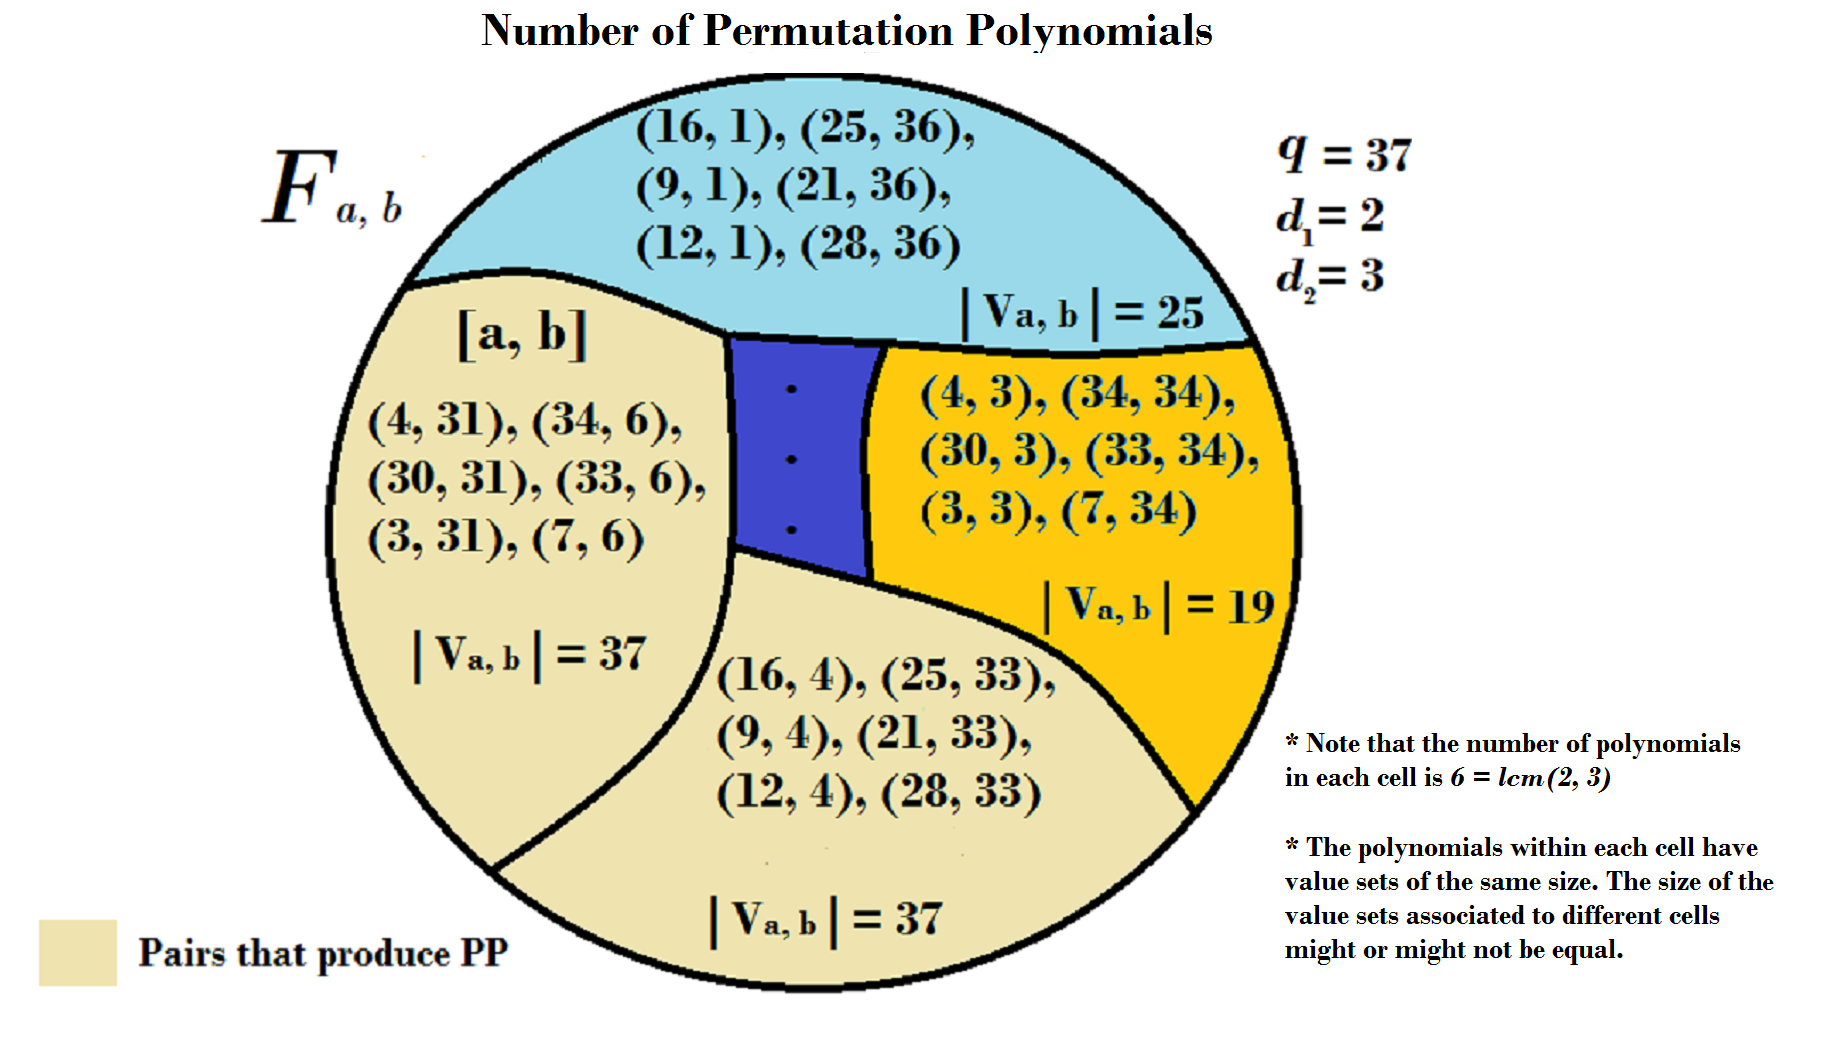
\includegraphics[width=11cm, height=6cm]{clases}
  \caption{A complete set of pairs $(a,b)$}
\end{figure}


%%%%%%%%%%%%%%%%%%%%
\section{Ongoing work}    
%%%%%%%%%%%%%%%%%%%%
    
    We have presented a class of trinomials that we expect produce many permutation polynomials. We have also presented a way to construct polynomials, given one of this family, with value sets of the same cardinality. This construction allows us to produce more permutation polynomials once we are given one. We wish to expand this work in the following ways:
    \begin{itemize}
    \item Find necessary and sufficient conditions on the parameters $(a,b)$ such that $F_{a,b}(X) = X(X^{\frac{q-1}{d_1}} + aX^{\frac{q-1}{d_2}} +b)$ is a permutation polynomial.
    \item Study our results on the family of polynomials of the form $F_{a,b}(X) = X^m(X^{\frac{q-1}{d_1}} + aX^{\frac{q-1}{d_2}} +b)$
    \item Find necessary and sufficient conditions such that $V_{a,b} = \mathbb{F}_q$ and $V_{a,b}$ is of minimal cardinality.
    \item Collect data on number of permutation polynomials of this form for different values of $d_1$ and $d_2$ and compare results with number of permutation binomials.
  \end{itemize}

%%%%%%%%%%%%%%%%%%%%
\section{Acknowledgements}
%%%%%%%%%%%%%%%%%%%%

  This work has been supported by a grant from the Center of Undergraduate Research in Mathematics (CURM) from Brigham Young University. Travel funds were provided by the MAA and the University of Puerto Rico, Rio Piedras.
 
\begin{thebibliography}{}
      \bibitem{main} Panario, D., Mullen, G., \textit{Handbook of Finite Fields}. CRC Press (2013).
      \bibitem{main} Wan, D., Lidl, R. \textit{Permutation Polynomials of the Form $x^{r}f(x^{\frac{q-1}{d}})$ and Their Group Structure}. Mh. Math. 112, 149-163 (1991).
      \bibitem{main} Borges, H., Conceicao R. \textit{On the characterization of minimal value set polynomial}. Journal of Number Theory 133 (2013) 2021-2035.
    \end{thebibliography}

\end{document}

